\documentclass[border=10pt]{standalone}
\usepackage{pgfplots}
\pgfplotsset{compat=1.18}

\begin{document}
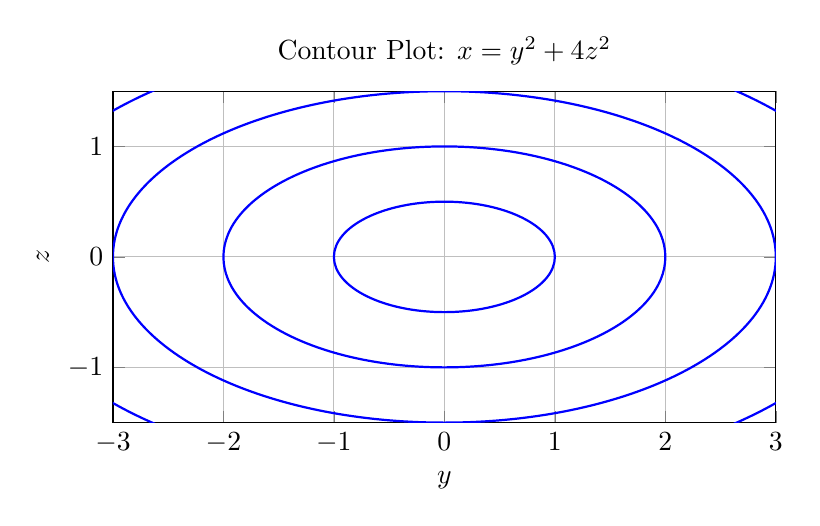
\begin{tikzpicture}
\begin{axis}[
    width=10cm,
    height=8cm,
    xlabel={$y$},
    ylabel={$z$},
    title={Contour Plot: $x = y^2 + 4z^2$},
    grid=major,
    xmin=-3,
    xmax=3,
    ymin=-1.5,
    ymax=1.5,
    axis equal image,
]
% Ellipses for different x values: y^2 + 4z^2 = k
% For k=1: y^2/1 + z^2/(1/4) = 1, so a=1, b=0.5
% For k=4: y^2/4 + z^2/1 = 1, so a=2, b=1
% For k=9: y^2/9 + z^2/(9/4) = 1, so a=3, b=1.5
\draw[blue, thick] (axis cs:0,0) ellipse [x radius=1, y radius=0.5];
\draw[blue, thick] (axis cs:0,0) ellipse [x radius=2, y radius=1];
\draw[blue, thick] (axis cs:0,0) ellipse [x radius=3, y radius=1.5];
\draw[blue, thick] (axis cs:0,0) ellipse [x radius=4, y radius=2];
\draw[blue, thick] (axis cs:0,0) ellipse [x radius=5, y radius=2.5];
\end{axis}
\end{tikzpicture}
\end{document}